\begin{appendix}

\section{Penman-Monteith}
\label{sec:penman}

\begin{description}
\item[Steigung der Sättigungsdampfdruckkurve]
\begin{equation}
\label{eq:delta}
\Delta=\frac{4098\left[0.6108*e^{\frac{17.27*T}{T+237.3}}\right]}{\left(T+237.3\right)^2}
\end{equation}
\begin{table}[H]
\centering
\begin{tabular}{ll}
$\mathrm{\Delta}$ & Steigung der Sättigungsdampfdruckkurve $\mathrm{[kPa/^{\circ}C]}$\\
T & mittlere Temperatur in 2\,m Höhe $\mathrm{[^{\circ}C]}$\\
\end{tabular}
\end{table}

\item[Nettostrahlung]

\begin{figure}[H]
\centering
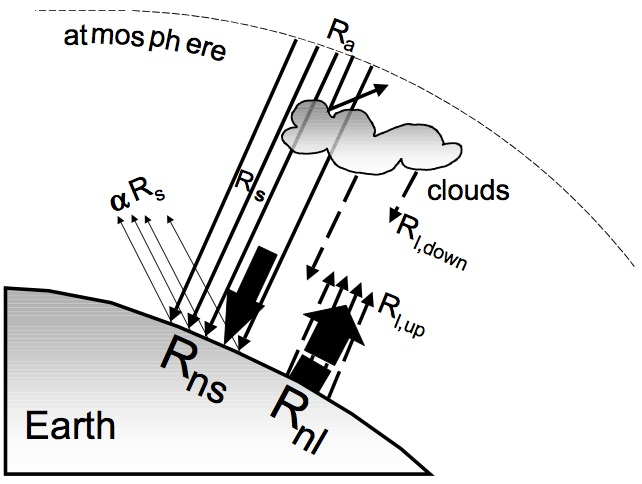
\includegraphics[width=0.8\textwidth]{figures/strahlung.jpg}
\caption{Schematische Darstellung der unterschiedlichen Strahlungsarten. $\mathrm{R_{s}}$ ist die kurzwellige Strahlung, $\mathrm{R_{l}}$ die langwellige Strahlung und $\mathrm{R_{a}}$ die atmosphärische Strahlung (aus \cite{fao})}
\label{fig:strahlung}
\end{figure}

\begin{equation}
\label{eq:rn}
R_n=0.77*R_s-\sigma\left[\frac{T_{max,K}^4+T_{min,K}^4}{2}\right]\left(0.34-0.14\sqrt{e_a}\right)\left(1.35\frac{R_s}{R_{s0}}-0.35\right)
\end{equation}
\begin{table}[H]
\centering
\begin{tabular}{ll}
$\mathrm{R_n}$ & Nettostrahlung $\mathrm{[MJ/m^2d]}$ \\
$\mathrm{R_s}$ & Kurzwellenstrahlung $\mathrm{[MJ/m^2d]}$ \\
$\mathrm{\sigma}$ & Stefan Boltzmann Konstante $\mathrm{[4.903*10^{-9}\,MJ/K^4m^2d]}$\\
$\mathrm{T_{max,K}}$ & maximale Temperatur während 24 h [K]\\
$\mathrm{T_{min,K}}$ & minimale Temperatur während 24 h [K]\\
$\mathrm{e_a}$ & aktueller Dampfdruck [kPa]\\
$\mathrm{R_{s0}}$ & Kurzwellenstrahlung ohne Wolkenbedeckung $\mathrm{[MJ/m^2d]}$\\
\end{tabular}
\end{table}

\begin{equation}
\label{eq:rs0}
R_{s0}=\left(0.75+2*10^{-5}z\right)*R_a
\end{equation}
\begin{table}[H]
\centering
\begin{tabular}{ll}
$\mathrm{R_s0}$ & Kurzwellenstrahlung ohne Wolkenbedeckung $\mathrm{[MJ/m^2d]}$\\
$\mathrm{R_a}$ & extraterrestrische Strahlung $\mathrm{[MJ/m^2d]}$ \\
z & Höhe über Meer [m]\\
\end{tabular}
\end{table}

\begin{equation}
\label{eq:Ra_short_period}
R_{a}=\frac{12 (60)}{\pi}G_{sc}*d_{r}[(\omega _{2}-\omega _{1})sin(\varphi)sin(\delta)+cos(\varphi)cos(\delta)(sin(\omega _{2})- sin(\omega _{1}))]
\end{equation}
\begin{table}[H]
\centering
\begin{tabular}{ll}
R$\mathrm{_{a}}$ & extraterrestrische Strahlung in einer Stunde (oder in kürzerem Zeitintervalll) [MJ/m$\mathrm{^{2}}$h]\\
G$\mathrm{_{sc}}$ & Solarkonstante = 0.0820 MJ/m$\mathrm{^{2}}$min\\
d$\mathrm{_{r}}$ & inverse relative Distanz Sonne-Erde\\
$\mathrm{\delta}$ & solare Deklination [rad]\\
$\mathrm{\varphi}$ & geografische Breite [rad]\\
$\mathrm{\omega_{1}}$ & Sonneneinstrahlwinkel am Anfang der Zeitperiode [rad]\\
$\mathrm{\omega_{2}}$ & Sonneneinstrahlwinkel am Ende der Zeitperiode [rad]\\
\end{tabular}
\end{table}

\begin{equation}
\label{eq:Ra_long_period}
R_{a}=\frac{24 (60)}{\pi}G_{sc}*d_{r}[\omega _{s}sin(\varphi)sin(\delta)+cos(\varphi)cos(\delta)sin(\omega _{s})]
\end{equation}
\begin{table}[H]
\centering
\begin{tabular}{ll}
R$\mathrm{_{a}}$ & extraterrestrische Strahlung in einem Tag (oder in längerem Zeitintervalll) [MJ/m$\mathrm{^{2}}$d]\\
G$\mathrm{_{sc}}$ & Solarkonstante = 0.0820 MJ/m$\mathrm{^{2}}$min\\
d$\mathrm{_{r}}$ & inverse relative Distanz Sonne-Erde [m]\\
$\mathrm{\delta}$ & solare Deklination [rad]\\
$\mathrm{\varphi}$ & geografische Breite [rad]\\
$\mathrm{\omega_{s}}$ & Sonneneinstrahlwinkel [rad]\\
\end{tabular}
\end{table}

\begin{equation}
\label{eq:dr}
d_r=1+0.033cos\left(\frac{2\pi}{365}J\right)
\end{equation}
\begin{equation}
\label{eq:delta_radiation}
\delta=0.409sin\left(\frac{2\pi}{365}J-1.30\right)
\end{equation}
\begin{table}[H]
\centering
\begin{tabular}{ll}
$\mathrm{d_r}$ & inverse Distanz Sonne-Erde [m]\\
$\mathrm{\delta}$ & solare Deklination [rad]\\
J & Korrekturfaktor (siehe \cite{fao} Annex 2 Table 2.5)\\
\end{tabular}
\end{table}

\begin{equation}
\label{eq:omega_s}
\omega_s=arccos[-tan(\varphi)tan(\delta)]
\end{equation}
\begin{table}[H]
\centering
\begin{tabular}{ll}
$\mathrm{\omega_s}$ & Sonneneinstrahlwinkel [rad]\\
$\mathrm{\varphi}$ & geografische Breite [rad]\\
$\mathrm{\delta}$ & solare Deklination [rad]\\
\end{tabular}
\end{table}

\begin{equation}
\label{eq:omega_i}
\omega_1=\omega-\frac{\pi t_i}{24}
\end{equation}
\begin{equation}
\omega_2=\omega+\frac{\pi t_i}{24}
\end{equation}
\begin{table}[H]
\centering
\begin{tabular}{ll}
$\mathrm{\omega}$ & Sonneneinstrahlwinkel [rad]\\
$\mathrm{t_i}$ & Zeitintervalldauer [h]\\
\end{tabular}
\end{table}

\begin{equation}
\label{eq:omega}
\omega=\frac{\pi}{12}[(t+0.06667(L_z-L_m)+S_c)-12]
\end{equation}
\begin{table}[H]
\centering
\begin{tabular}{ll}
$\mathrm{\omega}$ & Sonneneinstrahlwinkel [rad]\\
t & Zeit [h]\\
$\mathrm{L_z}$ & Längengrad in der Mitte der Zeitzone [rad]\\
$\mathrm{L_m}$ & Längengrad des Messpunktes [rad]\\
$\mathrm{S_c}$ & saisonaler Korrekturfaktor [h]\\
\end{tabular}
\end{table}

\begin{equation}
\label{eq:s_c}
S_c=0.1645sin(2b)-0.1255cos(b)-0.025sin(b)
\end{equation}
\begin{equation}
b=\frac{2\pi(J-81)}{364}
\end{equation}
\begin{table}[H]
\centering
\begin{tabular}{ll}
$\mathrm{S_c}$ & saisonaler Korrekturfaktor [h]\\
J & Korrekturfaktor (siehe \cite{fao} Annex 2 Table 2.5)\\
\end{tabular}
\end{table}

\item[Psychrometerkonstante]
\begin{equation}
\label{eq:gamma}
\gamma=0.665*10^{-3} P
\end{equation}
\begin{table}[H]
\centering
\begin{tabular}{ll}
$\mathrm{\gamma}$ & Psychrometerkonstante $\mathrm{[kPa/^{\circ}C]}$\\
P & Atmosphärendruck [kPa]\\
\end{tabular}
\end{table}

\item[Windgeschwindigkeit in 2 m Höhe]
\begin{equation}
\label{eq:u2}
u_2=u_z\frac{4.87}{ln(67.8z-5.42)}
\end{equation}
\begin{table}[H]
\centering
\begin{tabular}{ll}
$\mathrm{u_2}$ & Windgeschwindigkeit in 2\,m Höhe $\mathrm{[m/s]}$\\
$\mathrm{u_z}$ & Windgeschwindigkeit in z\,m Höhe $\mathrm{[m/s]}$\\
z & Messhöhe [m]\\
\end{tabular}
\end{table}



\item[Sättigungsdampfdruck]
\begin{equation}
\label{eq:es}
e_s=\frac{e^{\circ}(T_{max})+e^{\circ}(T_{min})}{2}
\end{equation}
\begin{table}[H]
\centering
\begin{tabular}{ll}
$\mathrm{e_s}$ & mittlerer Sättigungsdampfdruck $\mathrm{[kPa]}$\\
$\mathrm{e^{\circ}}$ & Sättigungsdampfdruck bei Temperatur T $\mathrm{[kPa]}$\\
T & mittlere Temperatur in 2\,m Höhe $\mathrm{[^{\circ}C]}$\\
\end{tabular}
\end{table}

\begin{equation}
\label{eq:enull}
e^{\circ}(T)=0.6108*e^{\frac{17.27T}{T+273.3}}
\end{equation}
\begin{table}[H]
\centering
\begin{tabular}{ll}
$\mathrm{e^{\circ}(T)}$ & Sättigungsdampfdruck bei Temperatur T $\mathrm{[kPa]}$\\
T & mittlere Temperatur in 2\,m Höhe $\mathrm{[^{\circ}C]}$\\\end{tabular}
\end{table}


\item[aktueller Dampfdruck]
\begin{equation}
\label{eq:ea}
e_a=\frac{RH_{mittel}}{100}*e_s
\end{equation}
\begin{table}[H]
\centering
\begin{tabular}{ll}
$\mathrm{e_a}$ & aktueller Dampfdruck $\mathrm{[kPa]}$\\
$\mathrm{e_s}$ & mittlerer Sättigungsdampfdruck $\mathrm{[kPa]}$\\
$\mathrm{RH_{mittel}}$ & mittlere relative Luftfeuchtigkeit [\%]\\
\end{tabular}
\end{table}

\end{description}

\section{Korrelationskoeffizient}
\label{sec:korrelation}
$$Korrelationskoeffizient(X,Y)=\frac{\sum (x-\bar{x})(y-\bar{y})}{\sqrt{\sum (x-\bar{x})^2\sum (y-\bar{y})^2}} $$
\center mit $\bar{x}$ und $\bar{y}$ als Mittelwerte der Datenreihen

\begin{figure}[H]
\centering
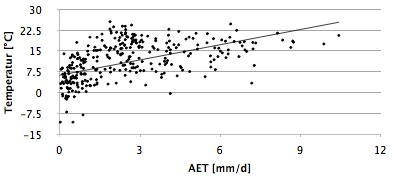
\includegraphics[width=0.8\textwidth]{figures/korr_temp.jpg}
\caption{grafische Darstellung der Korrelation zwischen der realen Evapotranspiration und der Temperatur}
\label{fig:korr_temp}
\end{figure}

\begin{figure}[H]
\centering
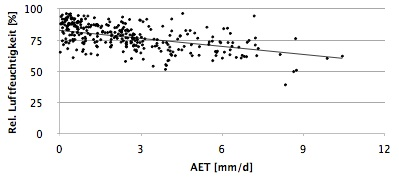
\includegraphics[width=0.8\textwidth]{figures/korr_relfeuchte.jpg}
\caption{grafische Darstellung der Korrelation zwischen der realen Evapotranspiration und der relativen Luftfeuchtigkeit}
\label{fig:korr_relfeucht}
\end{figure}

\begin{figure}[H]
\centering
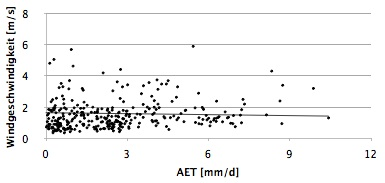
\includegraphics[width=0.8\textwidth]{figures/korr_windgeschw.jpg}
\caption{grafische Darstellung der Korrelation zwischen der realen Evapotranspiration und der Windgeschwindigkeit}
\label{fig:korr_wind}
\end{figure}

\begin{figure}[H]
\centering
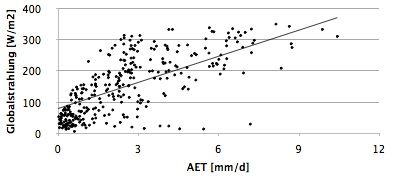
\includegraphics[width=0.8\textwidth]{figures/korr_globalstrahlung.jpg}
\caption{grafische Darstellung der Korrelation zwischen der realen Evapotranspiration und der Globalstrahlung}
\label{fig:korr_globalstrahlung}
\end{figure}

\section{potentielle Evapotranspiration}
\label{sec:Zeitintervalllpet}

\begin{figure}[H]
\centering
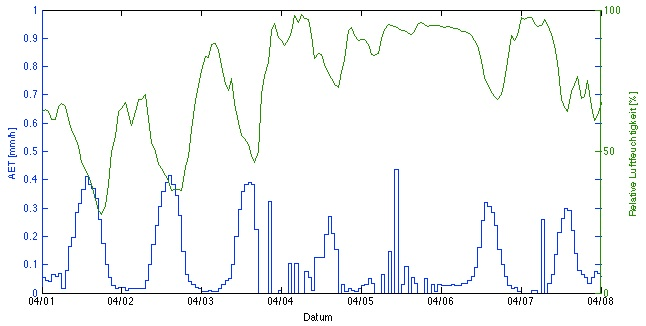
\includegraphics[width=0.8\textwidth]{figures/lys1_aet_feuchte_h.jpg}
\caption{grafische Darstellung der stündlichen PET und der relativen Luftfeuchtigkeit}
\label{fig:aet_feuchte}
\end{figure}

\begin{figure}[H]
\centering
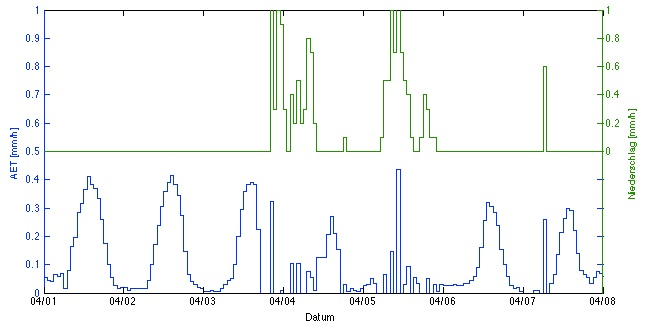
\includegraphics[width=0.8\textwidth]{figures/lys1_aet_niederschlag_h.jpg}
\caption{grafische Darstellung der stündlichen PET und des Niederschlag}
\label{fig:aet_niederschlag}
\end{figure}

\begin{figure}[H]
\centering
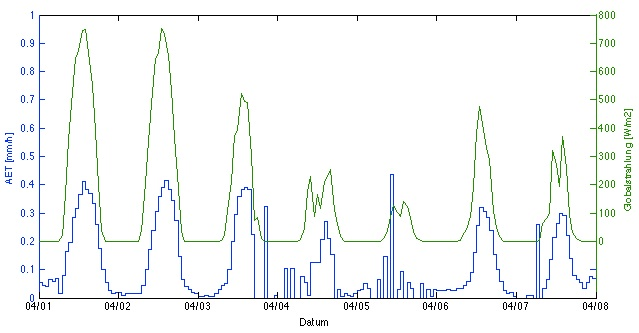
\includegraphics[width=0.8\textwidth]{figures/lys1_aet_strahlung_h.jpg}
\caption{grafische Darstellung der stündlichen PET und der Globalstrahlung}
\label{fig:aet_strahlung}
\end{figure}

\begin{figure}[H]
\centering
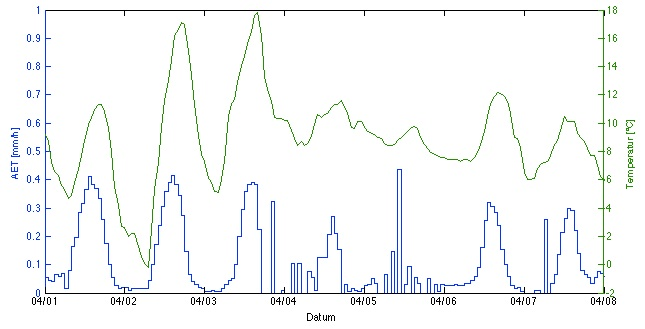
\includegraphics[width=0.8\textwidth]{figures/lys1_aet_temp_h.jpg}
\caption{grafische Darstellung der stündlichen PET und der Temperatur}
\label{fig:aet_temp}
\end{figure}

\begin{figure}[H]
\centering
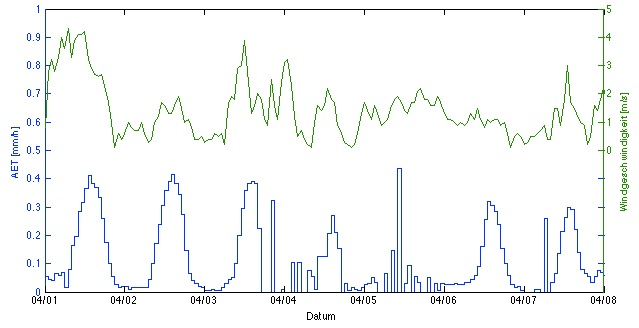
\includegraphics[width=0.8\textwidth]{figures/lys1_aet_wind_h.jpg}
\caption{grafische Darstellung der stündlichen PET und des Oberflächenwindes}
\label{fig:aet_wind}
\end{figure}

\section{Sensitivitätsanalyse}
\label{sec:sensitivitaet}

\begin{figure}[H]
\centering
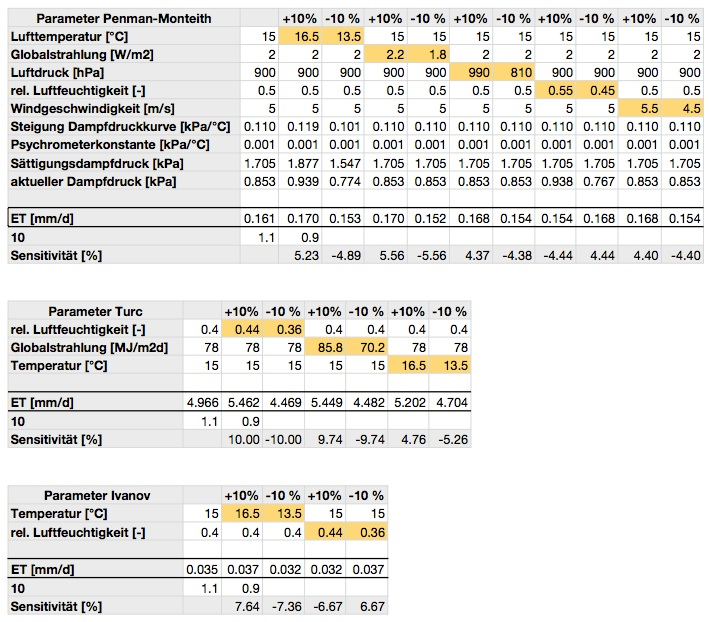
\includegraphics[width=0.8\textwidth]{figures/sensitivitaet.jpg}
\caption{tabellarische Berechnung der Sensitivität von der Penman-Monteith-, Turc- und Ivanov-Methode. Die markierten Felder wurden  verändert.}
\label{fig:sensitivitaet}
\end{figure}


\end{appendix}